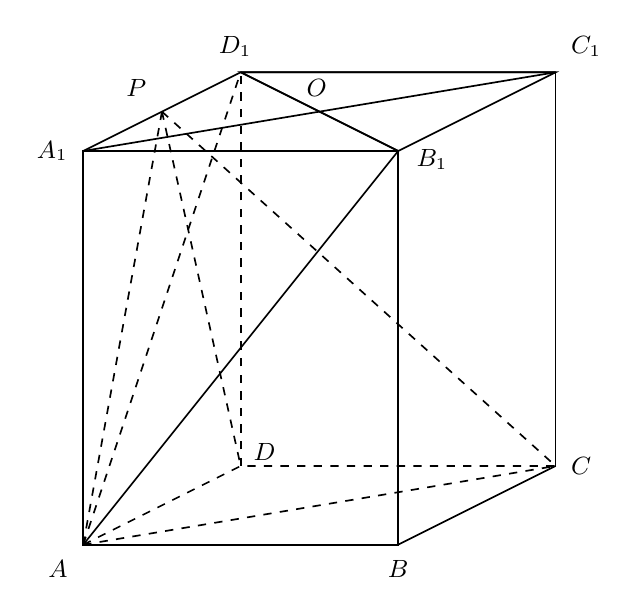
\begin{tikzpicture}[line width=.6pt,font=\small]
\coordinate (A) at (0,0);
\coordinate (B) at (4,0);
\coordinate (C) at (6,1);
\coordinate (D) at (2,1);
\coordinate (A1) at (0,5);
\coordinate (B1) at (4,5);
\coordinate (D1) at (2,6);
\coordinate (C1) at (6,6);
\coordinate (P) at (1.0000000000,5.5000000000);
\coordinate (O) at (3.0000000000,5.5000000000);
\draw (A) -- (B) -- (B1) -- (A1) -- cycle;
\draw (B) -- (C);
\draw (B1) -- (C1) -- (D1) -- cycle;
\draw (A1) -- (D1) -- (C1);
\draw (A1) -- (B1);
\draw (C1) -- (C);
\draw (A1) -- (C1);
\draw (D1) -- (B1);
\draw (A) -- (B1);
\draw[dashed] (A) -- (D) -- (C);
\draw[dashed] (D) -- (D1);
\draw[dashed] (A) -- (C);
\draw[dashed] (A) -- (P);
\draw[dashed] (P) -- (D);
\draw[dashed] (P) -- (C);
\draw[dashed] (A) -- (D1);
\node[below left,xshift=-2pt,yshift=-2pt] at (A) {$A$};
\node[below,xshift=0.0pt,yshift=-2pt] at (B) {$B$};
\node[right,xshift=2pt] at (C) {$C$};
\node[right,xshift=1pt,yshift=5pt] at (D) {$D$};
\node[left,xshift=-2pt] at (A1) {$A_{1}$};
\node[right,xshift=3pt,yshift=-3pt] at (B1) {$B_{1}$};
\node[above right,xshift=2pt,yshift=2pt] at (C1) {$C_{1}$};
\node[above,xshift=-2.0pt,yshift=2pt] at (D1) {$D_{1}$};
\node[above left,xshift=-2pt,yshift=2pt] at (P) {$P$};
\node[above,yshift=2pt,xshift=-1.0pt] at (O) {$O$};
\end{tikzpicture}
